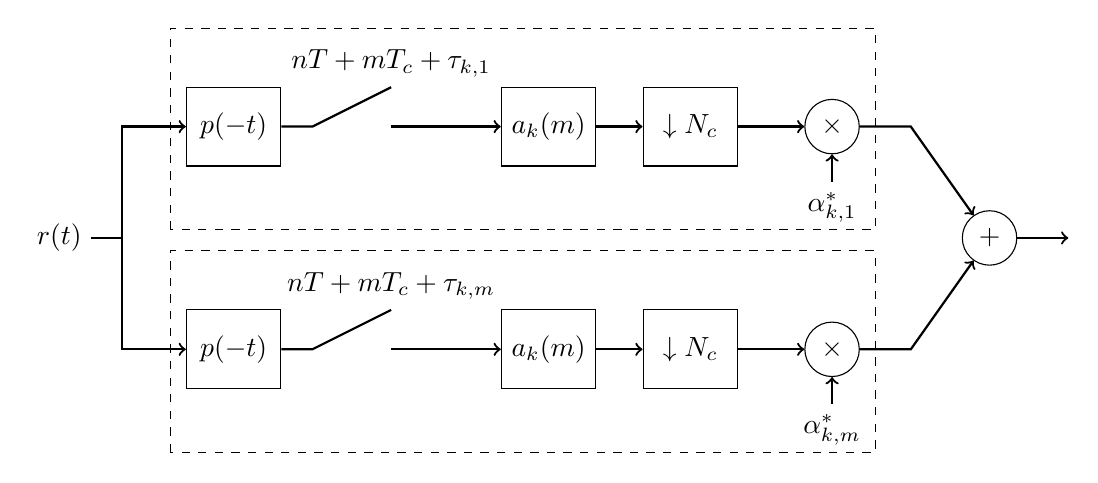
\begin{tikzpicture}
    \node (rt) {$r(t)$};

    \path (rt) -- ++(.8,0) coordinate (mrt);

    \node[above right of=mrt, draw, minimum width=1.2cm, minimum height=1cm, node distance=2cm] (p1) {$p(-t)$};
    \node[right of=p1, node distance=2cm] (split1) {};
    \node[right of=split1, draw, minimum width=1.2cm, minimum height=1cm, node distance=2cm] (a1) {$a_k(m)$};
    \node[right of=a1, draw, minimum width=1.2cm, minimum height=1cm, node distance=1.8cm] (up1) {$\downarrow N_c$};
    \node[right of=up1, draw, circle, node distance=1.8cm] (mul1) {$\times$};
    \draw[->, thick] (rt) -- (mrt) |- (p1);
    \draw[-, thick] (p1) -- ++(1,0) -- ([yshift=.5cm]split1.center) node[above] {$nT + m T_c + \tau_{k,1}$};
    \draw[->, thick] (split1.center) -- (a1);
    \draw[->, thick] (a1) -- (up1);
    \draw[->, thick] (up1) -- (mul1);
    \draw[dashed] ([shift={(-.2,-.8)}]p1.south west) rectangle ([shift={(+.3,+1)}]mul1.north east);
    \draw[<-,thick] (mul1) -- ++(0,-.7) node[below] {$\alpha_{k,1}^*$};

    \node[below right of=mrt, draw, minimum width=1.2cm, minimum height=1cm, node distance=2cm] (pm) {$p(-t)$};
    \node[right of=pm, node distance=2cm] (splitm) {};
    \node[right of=splitm, draw, minimum width=1.2cm, minimum height=1cm, node distance=2cm] (am) {$a_k(m)$};
    \node[right of=am, draw, minimum width=1.2cm, minimum height=1cm, node distance=1.8cm] (upm) {$\downarrow N_c$};
    \node[right of=upm, draw, circle, node distance=1.8cm] (mulm) {$\times$};
    \draw[->, thick] (rt) -- (mrt) |- (pm);
    \draw[-, thick] (pm) -- ++(1,0) -- ([yshift=.5cm]splitm.center) node[above] {$nT + m T_c + \tau_{k,m}$};
    \draw[->, thick] (splitm.center) -- (am);
    \draw[->, thick] (am) -- (upm);
    \draw[->, thick] (upm) -- (mulm);
    \draw[dashed] ([shift={(-.2,-.8)}]pm.south west) rectangle ([shift={(+.3,+1)}]mulm.north east);
    \draw[<-,thick] (mulm) -- ++(0,-.7) node[below] {$\alpha_{k,m}^*$};

    \path (mul1) -- ++(2,0) coordinate (X);

    \node[circle,draw] (add) at (X |- rt) {$+$};
    \draw[->,thick] (add) -- ++(1,0);

    \draw[->,thick] (mul1) -- ++(1,0) -- (add);
    \draw[->,thick] (mulm) -- ++(1,0) -- (add);


\end{tikzpicture}
